\documentclass[a4paper,12pt]{article}

\usepackage{array}
\usepackage{amsmath}
\usepackage{amssymb}
\usepackage[utf8x]{inputenc}
\usepackage[T2A]{fontenc}
% \usepackage[russian, english]{babel}
\usepackage[english,russian]{babel}

% Опционно, требует  apt-get install scalable-cyrfonts.*
% и удаления одной строчки в cyrtimes.sty
% Сточку не удалять!
% \usepackage{cyrtimes}

% Картнки и tikz
\usepackage{graphicx}


% Некоторая русификация.
\usepackage{misccorr}
\usepackage{indentfirst}
\renewcommand{\labelitemi}{\normalfont\bfseries{--}}
% Увы, костыль
% \addto\captionsrussian{\def\figurename{{\cyr\CYRR\cyri\cyrs\cyru\cyrn\cyro\cyrk}}}


% Увы, поля придётся уменьшить из-за листингов.
\topmargin -1cm
\oddsidemargin -0.5cm
\evensidemargin -0.5cm
\textwidth 17cm
\textheight 24cm

\sloppy

% Оглавление в PDF
\usepackage[
bookmarks=true,
colorlinks=true, linkcolor=black, anchorcolor=black, citecolor=black, menucolor=black,filecolor=black, urlcolor=black,
unicode=true
]{hyperref}



\title{ Методы вычислений \\Отчёт по лабораторной работе \textnumero 3 \\  }

\author{Кузьмин А.}
\date{24 мая 2013}

\begin{document}

%\maketitle

\begin{titlepage}
\newpage
\begin{center}
МГТУ им. Н.Э. Баумана \\		% \\ означает перенос
\hrulefill %горизонтальная черта
\end{center}

\vspace{10em}
\begin{center}
\Large Методы вычислений \\
\vspace{1em}
Отчет по лабораторной работе \textnumero 3
\end{center}


\begin{center}
\textsc{\textbf{Уравнение Пуассона}}
\end{center}

\vspace{15em}
\begin{flushright}
Кузьмин А. \\
Студент группы ИУ7-29 \\
Вариант 19
\end{flushright}
\vspace{\fill}
\begin{center}
Москва 2013
\end{center}
\end{titlepage}


\newpage

\section{Постановка задачи}
\subsection{Формулировка задачи}

Найти решение краевой задачи для уравнения Пуассона в прямоугольнике $0 \le x \le a$, $0 \le y \le b$ в следующей формулировке:

\[
\begin{array}{ll}
\bigtriangleup u + f = 0, \\
u \mid_{x=0} = \varphi_0(y), & u \mid_{y=0} = \psi_0(x), \\
u \mid_{x=a} = \varphi_a(y), & u \mid_{y=b} = \psi_b(x), \\
\end{array}
\]

Решение разностной задачи провести итерационным методом (верхней релаксации). Провести анализ указанной разностной схемы на устойчивость и сходимость. Оценить точность полученного решения. Для этого повторить вычисления, уменьшив вдвое шаг по каждой оси и сравнив результаты двух расчетов по совпадающим узлам.

Решение предоставить в табличном виде и графически.

\subsection{Исходные данные}

\newcolumntype{M}{>{\centering\arraybackslash}p{5cm}}
\newcolumntype{C}{>{\centering\arraybackslash}p{3cm}}
\newcolumntype{T}{>{\centering\arraybackslash}p{2cm}}

    \begin{tabular}{|C|M|}
        \hline
	 $a$ & 1 \\ \hline
	 $b$ & 1 \\ \hline
         $\varphi_0(y)$ & $2y^2$ \\ \hline
         $\varphi_a(y)$ & $2{sin(\pi y)}$ \\ \hline
         $\psi_0(x)$ & $x - x^2$ \\ \hline
         $\psi_b(x)$ & $2 - 2x$ \\ \hline
	 $f(x, y)$ & $5 + x + y$ \\ \hline
    \end{tabular}


\newpage
\section{Теоретические сведения}

Выбирается сетка с узлами $(x_i,t_j), i, j=\overline{0,N}, x_i=ih_x, t_j=jh_y $. Разностная схема строится, аппроксимируя частные производные 2-го порядка вторыми разностями. Пусть $u_{ij}$ = $u(x_i, y_j), f_{ij} = f(x_i, y_j)$. Тогда 

\begin{equation}
 \frac{u_{i-1,j} - 2u_{i,j} + u_{i+1,j}}{h_x^2} + \frac{u_{i,j-1} - 2u_{i,j} + u_{i,j+1}}{h_y^2} + f_{ij} = 0\\
\end{equation}

\begin{equation}
u_{0j} = \varphi_0(y_j), u_{Nj} = \varphi_a(y_j), u_{i0} = \psi_0(x_i), u_{iN} = \psi_b(x_i)\\
\end{equation}

\subsection{Метод верхней релаксации}
Решение задачи проводится методом верхней релаксации. Координатная форма метода имеет вид:


\begin{align*}
&u_{ij}^{k+1/2} = \frac{h_y^2}{2(h_x^2 + h_y^2)}(u_{i-1,j}^{k+1} + u_{i+1,j}^k) + 
	  							\frac{h_x^2}{2(h_x^2 + h_y^2)}(u_{i,j-1}^{k+1} + u_{i,j+1}^k) +
								  \frac{h_x^2 h_y^2}{2(h_x^2 + h_y^2)} f_{ij}, \\
&u_{ij}^{k+1} = \omega u_{ij}^{k+1/2} + (1-\omega)u_{ij}^k
\end{align*}

Значение параметра для метода верхней релаксации:

$$
\omega = \frac{2}{1+\sin\dfrac{\pi}{N}}
$$

\subsection{Условие останова}

Оценивать близость очередного приближения к точному решению проще оценивать по результатам последних двух итераций. В качестве условия останова используется неравенство:

$$
\|u^{k+1} - u^k\| < (2-\omega)\epsilon
$$

\section{Устойчивость}

Данная разностная схема "крест" является устойчивой. 

\section{Порядок аппроксимации}

В данном случае порядок аппроксимации равен $O(h_x^2 + h_y^2)$.
\newpage
\section{Результаты}

\begin{figure}[h]
\centering
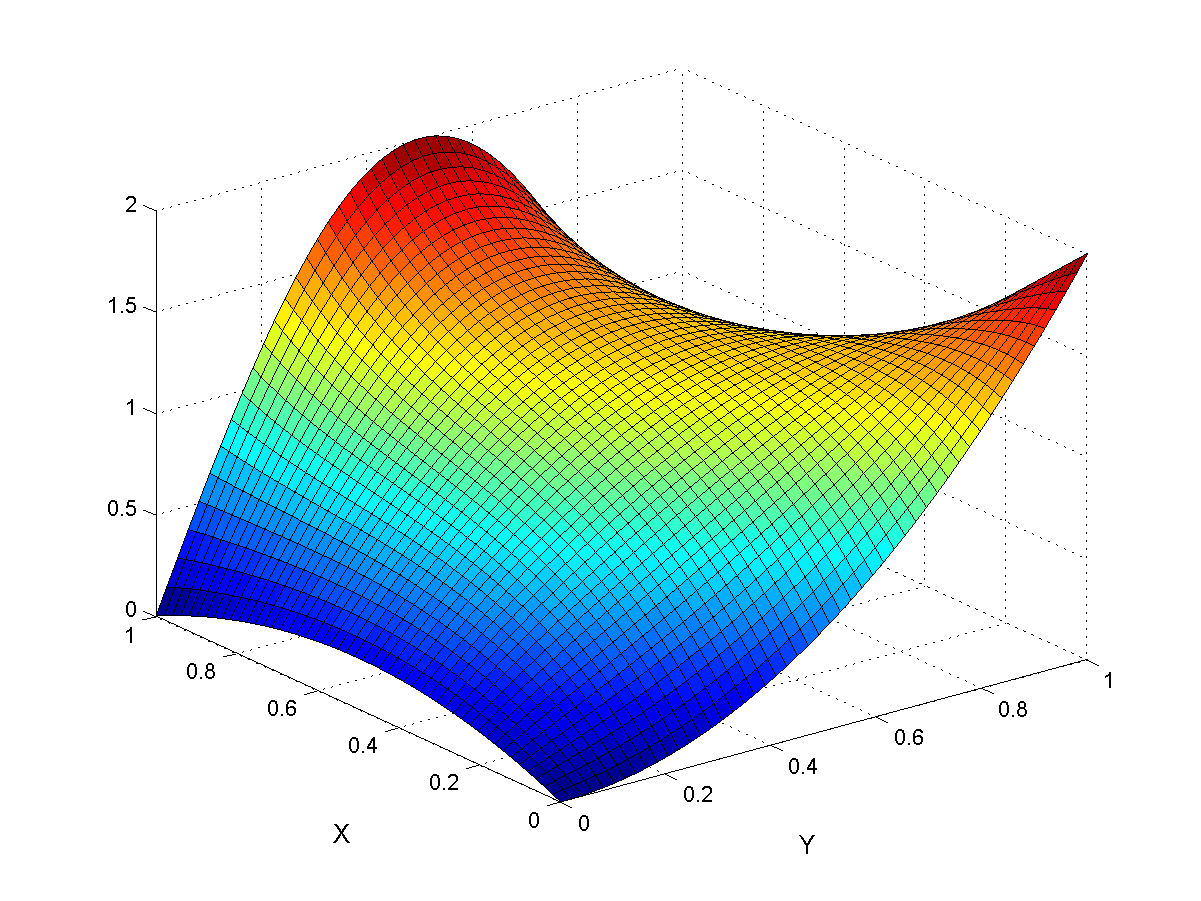
\includegraphics[width = 10cm]{screen.png}
\caption{Решение краевой задачи для уравнения Пуассона}
\label{fig:1}	
\end{figure}
\end{document}